\documentclass{article}
\usepackage{amsfonts, amsmath, amssymb, amsthm} % Math notations imported
\usepackage{enumitem}
\usepackage[margin=1in]{geometry}
\usepackage{graphicx}
\usepackage{subfig}
\graphicspath{{./images/}}

\newtheorem{thm}{Theorem}
\newtheorem{prop}[thm]{Proposition}
\newtheorem{cor}[thm]{Corollary}

% title information
\title{Math 180B HW1}
\author{Neo Lee}
\date{04/14/2023}

% main content
\begin{document} 

% placing title information; comment out if using fancyhdr
\maketitle 

\textbf{Problem 1.} 
\begin{enumerate}[label=(\alph*)]
    \item 
    \begin{align}
        E[e^{tX}] & = \int_{-\infty}^{\infty}e^{tx} \cdot \frac{\lambda}{\Gamma (\alpha)}(\lambda x)^{\alpha-1}e^{-\lambda x}dx \nonumber \\
        & = \int_{0}^{\infty}e^{tx} \cdot \frac{\lambda}{\Gamma (\alpha)}(\lambda x)^{\alpha-1}e^{-\lambda x}dx \qquad (\because x > 0 \emph{ for Gamma Distribution}) \nonumber \\
        & = \int_{0}^{\infty}\frac{\lambda}{\Gamma (\alpha)}(\lambda x)^{\alpha-1}e^{-(\lambda - t)x}dx. \nonumber 
    \end{align}

    Let $u = (\lambda - t)x$ for u-substitution. 
    Then $\frac{du}{\lambda - t} = dx$, and 1) $u\rightarrow \infty$ when $t < \lambda$ and $x\rightarrow\infty$;
    2) $u\rightarrow -\infty$ when $t > \lambda$ and $x\rightarrow\infty$; 
    3) $u\rightarrow 0$ when $t = \lambda$.

    Hence, when $t < \lambda$,
    \begin{align}
        E[e^{tX}] & = \int_{0}^{\infty}\frac{\lambda}{\Gamma (\alpha)}(\lambda \frac{u}{\lambda-t})^{\alpha-1}e^{-u}\frac{u}{\lambda-t} \nonumber \\
        & = \left(\frac{\lambda}{\lambda-t}\right)^\alpha \cdot \frac{1}{\Gamma (\alpha)}\int_{0}^{\infty}u^{\alpha-1}e^{-u}du \nonumber \qquad (\emph{notice} \int_{0}^{\infty}u^{\alpha-1}e^{-u}du = \Gamma (\alpha)) \\
        & = \left(\frac{\lambda}{\lambda-t}\right)^\alpha. \nonumber
    \end{align}

    When $t = \lambda$, $\lambda - t =0$, and 
    \begin{align}
        E[e^{tX}] & = \left(\frac{\lambda}{\lambda-t}\right)^\alpha \cdot \frac{1}{\Gamma (\alpha)}\int_{0}^{0}u^{\alpha-1}e^{-u}du \nonumber \\
        & = \left(\frac{\lambda}{\lambda-t}\right)^\alpha \cdot \frac{1}{\Gamma (\alpha)} \nonumber \\
        & = \lim_{t \rightarrow \lambda} \left(\frac{\lambda}{\lambda-t}\right)^\alpha \cdot \frac{1}{\Gamma (\alpha)} \nonumber \\
        & = \infty. \nonumber
    \end{align}

    When $t > \lambda$,
    \begin{align}
        E[e^{tX}] & = \left(\frac{\lambda}{\lambda-t}\right)^\alpha \cdot \frac{1}{\Gamma (\alpha)}\int_{0}^{-\infty}u^{\alpha-1}e^{-u}du \nonumber \qquad (\emph{notice}\int_{0}^{-\infty}u^{\alpha-1}e^{-u}du \emph{ diverges})\\
        & = \infty. \nonumber
    \end{align}

    Hence, we have reached the moment generating function of Gamma Distribution for all cases.

    \item
    Since we only care about $t=0$ and $\lambda > 0$, we can consider $M_X(t) = \left(\frac{\lambda}{\lambda-t}\right)^\alpha$ when $t < \lambda$ only.
    \begin{align}
        M_X'(t) & = \alpha\left(\frac{\lambda}{\lambda-t}\right)^{\alpha-1}\left(\frac{-\lambda}{(\lambda-t)^2}\right)(-1) \nonumber \\
        & = \alpha\left(\frac{\lambda}{\lambda-t}\right)^{\alpha}\left(\frac{1}{\lambda-t}\right) \nonumber \\
        & = \alpha \cdot \lambda^\alpha\cdot(\lambda-t)^{-\alpha-1} \nonumber \\
        \mu & = M_X'(t=0) = \frac{\alpha}{\lambda}. \nonumber \\
        M_X''(t) & = \alpha \cdot \lambda^\alpha\cdot (-\alpha-1)(\lambda-t)^{-\alpha-2}\cdot(-1) \nonumber \\
        & = \alpha \cdot \lambda^\alpha\cdot (\alpha+1)(\lambda-t)^{-\alpha-2} \nonumber \\
        \sigma^2 & = M_X''(t=0) = \frac{\alpha(\alpha+1)}{\lambda^2}. \nonumber
    \end{align}
\end{enumerate}
\bigbreak

\textbf{Problem 2.} 
\begin{align}
    \vec{\mu}=
    \begin{bmatrix}
        \mu_1 \\
        \mu_2
    \end{bmatrix}; \quad
    \Sigma=
    \begin{bmatrix}
        \sigma_1^2 & \rho\sigma_1\sigma_2 \\
        \rho\sigma_1\sigma_2 & \sigma_2^2
    \end{bmatrix}; \quad
    \vec{A_1}=
    \begin{bmatrix}
        1 \\
        2 
    \end{bmatrix}; \quad
    \vec{A_2}=
    \begin{bmatrix}
        1 \\
        -1
    \end{bmatrix}. \nonumber
\end{align}

Then 
\begin{align}
    Y_1 & \sim N(\vec{A_1}\cdot\vec{\mu}, A_1^{^\top}\sum A_1) \nonumber \\
    & = N(\mu_1+2\mu_2, \sigma_1^2+4\rho\sigma_1\sigma_2+4\sigma_2^2), \nonumber \\
    Y_2 & \sim N(\vec{A_2}\cdot\vec{\mu}, A_2^{^\top}\sum A_2) \nonumber \\
    & = N(\mu_1-\mu_2,\sigma_1^2-2\rho\sigma_1\sigma_2+\sigma_2^2). \nonumber
\end{align}

The $pdf$ of a normal random variable $N(m,s)$ for all $x \in \mathbb{R}$ is simply 
\begin{align}
    f(x) = \frac{1}{\sqrt{2\pi s}}e^{-\frac{(x-m)^2}{2s}}. \nonumber
\end{align}
Since we have already found the mean and variance of $Y_1$ and $Y_2$, and we have determined they are normal random variable, what's left is only plugging into the formula, which we will omit here for easier readability as a whole.
\bigbreak

\textbf{PK Problem 2.1.8} 
Let $F$ be first ball, $S$ be second ball.
\begin{align}
    P(F = R | S = R) & = \frac{P(S = R | F = R)P(F = R)}{P(S = R | F = R)P(F = R) + P(S = R | F = G)P(F = G)} \nonumber \\
    & = \frac{\frac{2}{3}\cdot\frac{1}{2}}{\frac{2}{3}\cdot\frac{1}{2} + \frac{1}{3}\cdot\frac{1}{2}} \nonumber \\
    & = \frac{2}{3}. \nonumber
\end{align}
\bigbreak

\textbf{PK Problem 2.1.9} 
\begin{align}
    p_N(n) & = \begin{cases}
        \frac{e^{-1}}{n!}, & n \in \mathbb{Z^{^\ge}}\nonumber \\
        0, & \text{otherwise}, \nonumber
    \end{cases} \\
    p_{X|N=n}(x) & = \begin{cases}
        \frac{1}{n+2}, & x \in [0,n+1] \nonumber \\
        0, & \text{otherwise}. \nonumber
    \end{cases}
\end{align}

Then, 
\begin{align}
    p_X(x) & = \sum_{n=x-1}^{\infty}p_{X|N=n}(x)\cdot p_N(n) \nonumber \\
    & = \sum_{n=x-1}^{\infty}\frac{1}{n+2} \cdot \frac{e^{-1}}{n!} \nonumber \\
    & = \frac{1}{e}\sum_{n=x-1}^{\infty}\frac{n+1}{(n+2)!} \nonumber \\
    & = \frac{1}{e}\sum_{n=x}^{\infty}\frac{n}{(n+1)!} \nonumber \\
    & = \frac{1}{e}\sum_{n=1}^{\infty}\frac{n}{(n+1)!} - \sum_{n=1}^{x-1}\frac{n}{(n+1)!} \nonumber \\
    & = \frac{1}{e}\left(1-\frac{x!-1}{x!}\right) \nonumber \\ 
    & = \frac{1}{e} + \frac{1-x!}{e\cdot x!}. \nonumber
\end{align}
\bigbreak

\textbf{PK Exercise 2.3.1} 
\underline{Random Sum approach:} Let $\xi_i \sim$ \emph{Bernoulli}$(\frac{1}{2})$, $Z = \xi_1 + \xi_2 + \dots + \xi_n$, and $N \sim $\emph{Uniform}$(1,6)$.
Then 
\begin{align}
    E[Z] & = E[\xi_i]E[N] \nonumber \\
    & = \frac{1}{2}\cdot\frac{7}{2}\nonumber \\
    & =\frac{7}{4}, \nonumber \\
    Var(Z) & = Var(\xi_i)E[N] + Var(N)(E[\xi_i])^2 \nonumber \\
    & = \frac{1}{4}\cdot\frac{7}{2} + \frac{6^2-1}{12}\cdot\left(\frac{1}{2}\right)^2 \nonumber \\
    & = \frac{77}{48}. \nonumber
\end{align}

\underline{\emph{pmf} approach:} Let $Z \sim \emph{Bionomial}(n,\frac{1}{2})$ and $N \sim \emph{Uniform}(1,6)$. 
Then 
\begin{align}
    p_Z(z) & = \sum\limits_{n=z}^6p_{Z|N=n}(z)p_N(n) \nonumber \\
    & = \sum\limits_{n=z}^6{n \choose z}\left(\frac{1}{2}\right)^n\cdot \frac{1}{6}, \nonumber \\
    E[Z] & =\sum\limits_{z=0}^6z\cdot p_Z(z) \nonumber \\
    & = \sum\limits_{z=0}^6z\cdot \left[\sum\limits_{n=z}^6{n \choose z}\left(\frac{1}{2}\right)^n\cdot \frac{1}{6}\right] \nonumber \\
    & = \frac{7}{4}, \nonumber \\
    Var(Z) & = E[Z^2] - (E[Z])^2 = \frac{14}{3} - \left(\frac{7}{4}\right)^2 \nonumber \\
    & = \frac{77}{48}. \nonumber
\end{align}
\begin{figure}[htb]
    \qquad
    \begin{minipage}{.4\textwidth}
        \centering
        {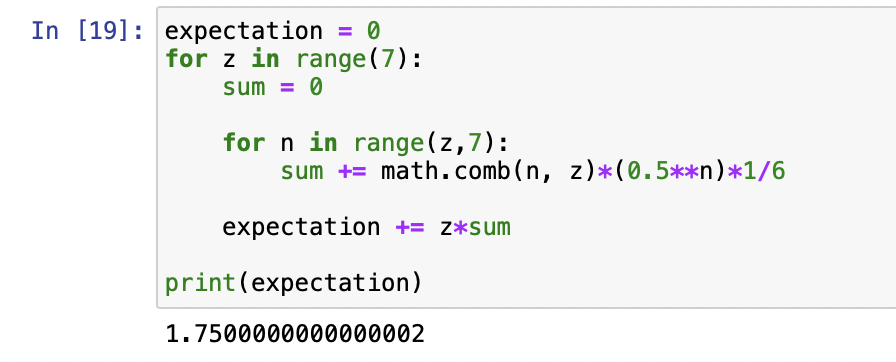
\includegraphics[scale=0.4]{E[Z].png}}
        \qquad\qquad$E[Z]$\label{fig:1}
    \end{minipage}    
    \qquad
    \begin{minipage}{.4\textwidth}
        \centering
        {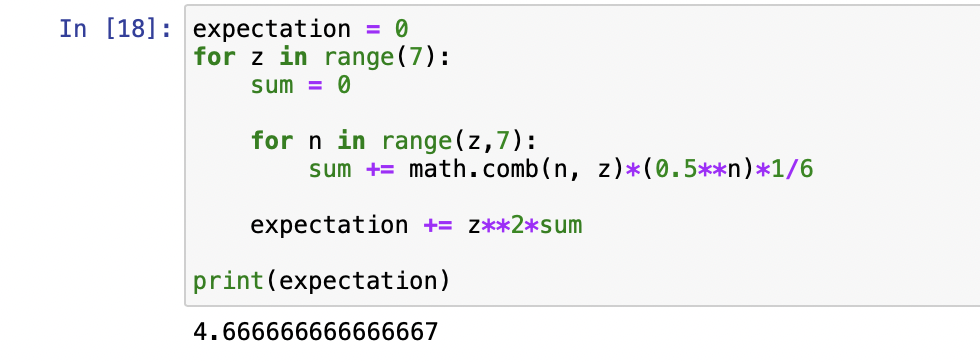
\includegraphics[scale=0.4]{E[Z^2].png}}
        \qquad\qquad$E[Z^2]$\label{fig:2}
    \end{minipage}        
\end{figure} 
\bigbreak

\textbf{PK Exercise 2.3.5} 
Let $N$ be a \emph{Poisson} random variable representing number of accidents in a week, 
and $\xi_i$ be a random variable representing the number of individuals injured in each accident (assume all $\xi_i$ are independent and identically distributed).
Then the number of individuals, $Z$, injued in a week can be written as $Z = \xi_1 + \xi_2 + \dots + \xi_n$.

Hence, 
\begin{align}
    E[Z] & = E[\xi_i]E[N] \nonumber \\
    & = 3 \times 2 \nonumber \\
    & = 6, \nonumber \\
    Var(Z) & = Var(\xi_i)E[N] + Var(N)(E[\xi_i])^2 \nonumber \\
    & = 4\times 2 + 2\times 9 \nonumber \\
    & = 26. \nonumber
\end{align}
\bigbreak

\end{document}